\documentclass[11pt]{article}

\usepackage[T1]{fontenc}
\usepackage{lmodern}
\usepackage[margin=1in]{geometry}
\usepackage{microtype}
\usepackage{amsmath,amssymb,amsthm,mathtools}
\usepackage{enumitem}
\usepackage{graphicx}
\usepackage[hidelinks]{hyperref}

\newtheorem{theorem}{Theorem}
\newtheorem{lemma}[theorem]{Lemma}
\newtheorem{proposition}[theorem]{Proposition}
\newtheorem{corollary}[theorem]{Corollary}
\theoremstyle{remark}
\newtheorem{remark}[theorem]{Remark}

\newcommand{\dens}{\operatorname{dens}}
\newcommand{\clspan}{\overline{\operatorname{span}}}
\newcommand{\one}{\mathbf 1}
\newcommand{\N}{\mathbb N}
\newcommand{\R}{\mathbb R}
\newcommand{\supp}{\operatorname{supp}}
\newcommand{\eqstar}{=^{*}}

\title{A ZFC Overcomplete Set in $C([0,\omega_1])$\\
with No Weak Cluster Point}
\author{Verification and problem exploration report}
\date{June 22, 2026}

\begin{document}
\maketitle

\begin{abstract}
Russo and Somaglia asked whether $C([0,\omega_1])$ contains an overcomplete
set with no weak cluster point, and whether (for example under CH) an
overcomplete set can be weakly discrete.  The supplied partial packet gives an
affirmative answer under CH.  We verify that argument, apart from a minor
net-selection detail that is easily repaired.

A literature search located Koszmider's later ZFC construction of an
overcomplete set in $C([0,\omega_1])$, but no published resolution of the
additional weak-topological requirement.  We then give a ZFC construction
which appears to settle both questions affirmatively.  In fact, for every
$0<\varepsilon<1/2$ we construct an overcomplete family
$(x_\alpha)_{\alpha<\omega_1}$ satisfying
\[
  \bigl\|x_\alpha-\one_{[0,\alpha]}\bigr\|<\varepsilon
  \qquad(\alpha<\omega_1).
\]
It follows that the family is norm separated and weakly closed-discrete.
The argument combines the almost coherent injections used in Koszmider's
nonseparable version of Klee's construction with a small analytic term whose
Taylor coefficients grow unboundedly.  This report is not peer reviewed, so
the proposed ZFC resolution should be independently checked before being
cited as established literature.
\end{abstract}

\section*{Packet status}

\begin{description}[leftmargin=2.8cm,style=nextline]
\item[Run] \texttt{fa\_banach\_001}.
\item[Source arXiv id] \texttt{1912.08690}.
\item[Source paper] T.~Russo and J.~Somaglia, \emph{Overcomplete sets in
non-separable Banach spaces}, arXiv:1912.08690.
\item[Packet classification] Candidate full solution, likely valid subject to
human mathematical review.
\item[Upgrade note] This packet supersedes the earlier CH partial packet for
the same source question.  The earlier packet is preserved in
\texttt{history/packets/}; the new theorem removes CH and gives a ZFC
weakly closed-discrete overcomplete set in \(C([0,\omega_1])\).
\end{description}

The source question appears in Section~4.1 of Russo--Somaglia:

\begin{center}
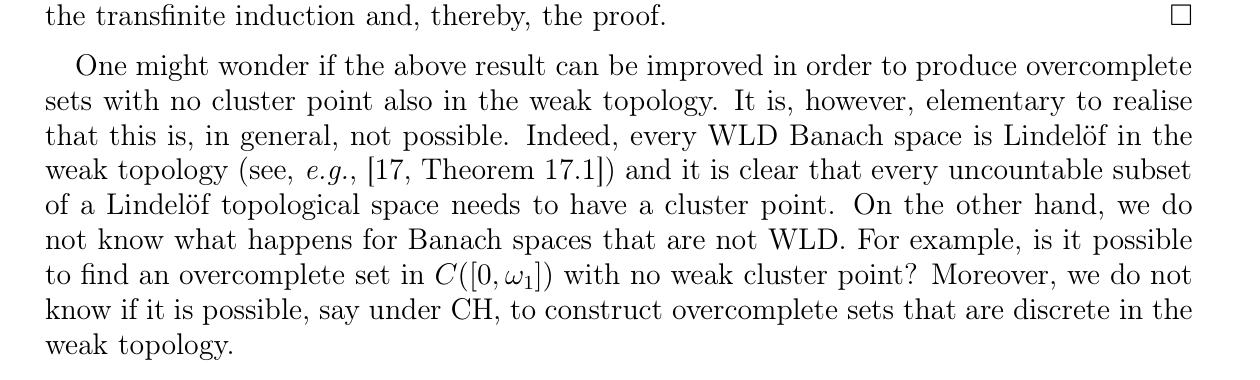
\includegraphics[width=\linewidth]{figures/open_question_page10_crop.png}
\end{center}

\section{The question and the status of the supplied partial result}

For a Banach space $X$, a set $S\subseteq X$ is \emph{overcomplete} if
$|S|=\dens X$ and every subset of $S$ having cardinality $|S|$ is linearly
dense in $X$.  Russo and Somaglia asked whether one can find an overcomplete
set in $C([0,\omega_1])$ with no weak cluster point.  They also asked whether,
say under CH, one can construct overcomplete sets which are discrete for the
weak topology \cite[Section 4.1]{RussoSomaglia}.

The supplied packet proposes the following CH argument.  Put
$u_\alpha=\one_{[0,\alpha]}$.  Small norm balls around the $u_\alpha$'s are
locally finite in the topology of pointwise convergence.  Under CH, enumerate
all hyperplanes of $C([0,\omega_1])$ in order type $\omega_1$ and choose, at
stage $\alpha$, a point close to $u_\alpha$ and outside all preceding
hyperplanes.  Every hyperplane then contains only countably many selected
points, which is exactly the hyperplane criterion for overcompleteness.

\begin{proposition}[Audit of the supplied packet]
The CH theorem in the supplied packet is correct.  Its local-finiteness
argument needs only the following minor clarification: failure of local
finiteness gives a net of indices which eventually avoids every finite subset
of $\omega_1$, rather than automatically a globally injective net.  That is
all the proof needs.  Moreover, the radius restriction can be improved from
$r<1/3$ to $r<1/2$.
\end{proposition}

\begin{proof}
The repaired local-finiteness proof is given in Lemma~\ref{lem:localfinite}
below.  Once that lemma is available, the CH recursion is standard.  At every
countable stage, a nonempty norm-open ball cannot be covered by countably many
hyperplanes and points, by the Baire category theorem.  If an uncountable
subfamily failed to be linearly dense, a nonzero functional would annihilate
it, so its kernel would be one of the enumerated hyperplanes and would contain
uncountably many selected points, contradicting the recursion.  Local
finiteness of the containing balls then makes the selected set weakly
closed-discrete.
\end{proof}

\section{Literature search}

The source problem appears in the 2021 paper of Russo and Somaglia
\cite{RussoSomaglia}.  Koszmider subsequently proved in ZFC that
$C([0,\omega_1])$ admits an overcomplete set \cite[Theorem 11]{Koszmider}; his
argument uses a coherent family of injections and a nonseparable analogue of
Klee's analytic construction.  That theorem settles plain existence, but its
statement and proof do not impose the absence of weak cluster points.  The
2022 hyperplane-covering follow-up \cite{GlodkowskiKoszmider} addresses a
different overcomplete-set problem.  Russo's 2025 habilitation overview still
summarizes this part of the theory through the original paper and the two
follow-ups, without recording a resolution of the weak-topological question
\cite[pp.~16--17]{RussoHab}.

Exact-phrase searches for the displayed question, ``weak cluster point'',
``weakly discrete'', and ``weakly closed-discrete'', together with searches of
the citation trail and current author publication lists, did not locate a
published proof or counterexample through June 22, 2026.  This is necessarily a
bounded novelty check, not a proof that no such result exists.

\section{Proof Intuition}

The old CH argument used a well ordering of all hyperplanes and chose points
near the clopen initial-segment functions \(u_\alpha=\one_{[0,\alpha]}\).
The ZFC construction replaces that global enumeration with a direct
functional-separation mechanism.

Every functional on \(C([0,\omega_1])\) has countable support, so its
cumulative values \(\mu(u_\alpha)\) are eventually constant.  The terms
\(u_\beta-u_\alpha\) cancel this eventual constant.  Almost coherent
injections then make the values of a fixed functional on an uncountable
subfamily into zeros of one analytic function.  The additional scalar term
\(q(r_\alpha)\one_K\), with \(q(t)=t/(1-2t)\), detects the remaining endpoint
mass at \(\omega_1\): its Taylor coefficients grow like \(2^n\), while the
coefficients coming from a bounded functional stay bounded.  Therefore a
nonzero functional cannot vanish on uncountably many constructed vectors.

The weak-topological control is kept by forcing
\(\|x_\alpha-u_\alpha\|<\varepsilon<1/2\).  Small balls around the
\(u_\alpha\)'s are weakly locally finite, so the final overcomplete set has no
weak cluster point and is weakly closed-discrete.

\section{Two preliminary lemmas}

Let
\[
  K=[0,\omega_1],\qquad X=C(K),\qquad
  u_\alpha=\one_{[0,\alpha]}\quad(\alpha<\omega_1).
\]
Each $[0,\alpha]$ is clopen, so $u_\alpha\in X$.  We first record the
weak-topological part of the supplied argument in a fully explicit form.

\begin{lemma}\label{lem:localfinite}
For every $0<r<1/2$, the family
\[
  \mathcal B_r=\{B(u_\alpha,r):\alpha<\omega_1\}
\]
is locally finite for the topology of pointwise convergence on $X$.
Consequently it is locally finite for the weak topology of $X$.
\end{lemma}

\begin{proof}
Suppose that $\mathcal B_r$ is not locally finite at some $f\in X$.  Direct the
pairs $(V,F)$, where $V$ is a pointwise neighbourhood of $f$ and
$F\subseteq\omega_1$ is finite, by refinement of $V$ and enlargement of $F$.
For every such pair choose
\[
  \alpha_{V,F}\notin F,
  \qquad
  g_{V,F}\in V\cap B(u_{\alpha_{V,F}},r).
\]
Then $g_{V,F}\to f$ pointwise, while the index net
$(\alpha_{V,F})$ eventually avoids every finite subset of $\omega_1$.

By compactness of $K$, pass to a subnet for which
$\alpha_{V,F}\to\lambda\in K$.  The subnet is not eventually constant.  Since
all isolated points of the ordinal compactum force eventually constant
convergence, $\lambda$ is a limit ordinal, possibly $\omega_1$.  A direct check
in the order topology gives
\[
  u_{\alpha_{V,F}}(t)\longrightarrow v_\lambda(t)
  \quad(t\in K),
  \qquad
  v_\lambda=\one_{[0,\lambda)}.
\]
Indeed, for $t<\lambda$ the indices are eventually above $t$, whereas at
$t=\lambda$ they are eventually strictly below $\lambda$; for $t>\lambda$ they
are eventually below $t$.

For every $t\in K$ we therefore have
\[
  |f(t)-v_\lambda(t)|\le r.
\]
In particular,
\[
  |f(\lambda)|\le r,
  \qquad
  |f(\xi)-1|\le r\quad(\xi<\lambda),
\]
so
\[
  |f(\xi)-f(\lambda)|\ge 1-2r>0
  \qquad(\xi<\lambda).
\]
This contradicts continuity of $f$ at the limit point $\lambda$.  Hence the
family is pointwise locally finite.  Since every coordinate evaluation
$\delta_t$ is weakly continuous, every pointwise neighbourhood used above is
also weakly open, and weak local finiteness follows.
\end{proof}

The combinatorial device below is standard and is used explicitly in
Koszmider's construction \cite[Lemma 9]{Koszmider}.  We include a proof for
completeness.  For two functions on a common domain, $p\eqstar q$ means that
they differ at only finitely many points.

\begin{lemma}[Almost coherent injections]\label{lem:coherent}
There are injections $e_\alpha:\alpha\to\N$ for $\alpha<\omega_1$ such that
\[
  e_\beta\!\upharpoonright\alpha\eqstar e_\alpha
  \qquad(\alpha<\beta<\omega_1).
\]
They may moreover be chosen so that $\N\setminus e_\alpha[\alpha]$ is infinite
for every $\alpha$.
\end{lemma}

\begin{proof}
Proceed by transfinite recursion.  At a successor stage, extend $e_\alpha$ by
sending the new point to an unused integer; the infinite-complement condition
is preserved.

Let $\lambda<\omega_1$ be a limit ordinal, and choose an increasing cofinal
sequence $(\lambda_n)_{n<\omega}$ in $\lambda$.  Recursively construct
injections $h_n:\lambda_n\to\N$ so that $h_{n+1}$ extends $h_n$ and
$h_n\eqstar e_{\lambda_n}$.  To pass from $n$ to $n+1$, use
$e_{\lambda_{n+1}}$ on the new block
$\lambda_{n+1}\setminus\lambda_n$.  Only finitely many of those values collide
with $h_n[\lambda_n]$, because
$h_n\eqstar e_{\lambda_{n+1}}\!\upharpoonright\lambda_n$; alter those finitely
many values to fresh integers.  There are infinitely many available integers,
since the union in question is a finite perturbation of
$e_{\lambda_{n+1}}[\lambda_{n+1}]$.

Set $h=\bigcup_n h_n$.  Then $h$ is injective and
$h\!\upharpoonright\lambda_n\eqstar e_{\lambda_n}$ for every $n$.  If the
complement of $h[\lambda]$ is not infinite, choose a countable set
$B=\{\xi_n:n<\omega\}\subseteq\lambda$ such that
$B\cap\lambda_m$ is finite for every $m$ (take $\xi_n\ge\lambda_n$), partition
$B$ into infinitely many infinite sequences, and on each sequence shift the
$h$-values forward by one place.  This preserves injectivity, changes $h$ only
finitely often on every $\lambda_m$, and frees one value from each sequence.
The resulting injection is $e_\lambda$.  Coherence with every earlier ordinal
follows from cofinality of $(\lambda_n)$ and transitivity of $\eqstar$.
\end{proof}

\begin{corollary}[Exact stabilization on an initial segment]\label{cor:stabilize}
Let $(e_\alpha)$ be as in Lemma~\ref{lem:coherent}.  If
$A\subseteq\omega_1$ is uncountable and $\gamma<\omega_1$, then there are an
uncountable $A'\subseteq A\setminus(\gamma+1)$ and an injection
$g:\gamma+1\to\N$ such that
\[
  e_\alpha\!\upharpoonright(\gamma+1)=g
  \qquad(\alpha\in A').
\]
\end{corollary}

\begin{proof}
For $\alpha>\gamma$, the restriction
$e_\alpha\!\upharpoonright(\gamma+1)$ differs from $e_{\gamma+1}$ on a finite
set.  Since $\gamma+1$ is countable, there are only countably many finite
subsets of it; thin $A$ to an uncountable set on which that exceptional set is
fixed.  There are only countably many maps from the fixed finite exceptional
set into $\N$, so a second thinning makes the entire restriction constant.
\end{proof}

\section{The ZFC construction}

The key design is as follows.  For a functional $\mu$, the cumulative values
$\mu(u_\alpha)$ are eventually constant, because $\mu$ has countable support.
The differences $u_\beta-u_\alpha$ cancel that eventual constant.  The
coherent injections then turn evaluation on an uncountable subfamily into the
zero set of one analytic function.  Those differences all vanish at
$\omega_1$, however, so an extra constant-vector term is needed to detect the
atom at $\omega_1$.  We choose that term to have unbounded Taylor coefficients,
whereas all coefficients coming from a bounded functional remain uniformly
bounded.

\begin{theorem}[ZFC]\label{thm:main}
For every $0<\varepsilon<1/2$, there is a family
$S=\{x_\alpha:\alpha<\omega_1\}\subseteq C([0,\omega_1])$ such that
\begin{enumerate}[label=\textup{(\roman*)},leftmargin=2.2em]
\item $\|x_\alpha-u_\alpha\|<\varepsilon$ for every $\alpha<\omega_1$;
\item for every nonzero $\mu\in C([0,\omega_1])^*$, the set
      $\{\alpha<\omega_1:\mu(x_\alpha)=0\}$ is countable.
\end{enumerate}
Consequently $S$ is overcomplete, bounded, $(1-2\varepsilon)$-separated in
norm, and weakly closed-discrete.  In particular, $S$ has no weak cluster
point.
\end{theorem}

\begin{proof}
Fix $b\in(0,1/2)$ so small that
\begin{equation}\label{eq:smallb}
  \frac{b}{1-b}+\frac{b}{1-2b}<\varepsilon.
\end{equation}
Choose pairwise distinct numbers
$r_\alpha\in[b/2,b]$ for $\alpha<\omega_1$; this is possible because every
nondegenerate real interval has cardinality $\mathfrak c\ge\omega_1$.  Let
$(e_\alpha)_{\alpha<\omega_1}$ be as in Lemma~\ref{lem:coherent}, and put
\[
  q(t)=\frac{t}{1-2t}=\sum_{n=0}^{\infty}2^n t^{n+1}
  \qquad(|t|<1/2).
\]
For $\alpha<\omega_1$, define
\begin{align}
  w_\alpha
    &=\sum_{\beta<\alpha}
      r_\alpha^{\,e_\alpha(\beta)+1}(u_\beta-u_\alpha),
      \label{eq:walpha}\\
  x_\alpha
    &=u_\alpha+w_\alpha+q(r_\alpha)\one_K.
      \label{eq:xalpha}
\end{align}
The series in \eqref{eq:walpha} converges absolutely in norm, since
$e_\alpha$ is injective and $\|u_\beta-u_\alpha\|=1$ for $\beta<\alpha$.
Moreover,
\[
  \|w_\alpha\|
  \le\sum_{n=0}^{\infty}r_\alpha^{n+1}
  =\frac{r_\alpha}{1-r_\alpha}
  \le\frac b{1-b}.
\]
Together with \eqref{eq:smallb}, this gives
\[
  \|x_\alpha-u_\alpha\|
  \le \frac b{1-b}+\frac b{1-2b}<\varepsilon,
\]
which proves (i).

We prove (ii).  Since $K$ is scattered, every functional on $C(K)$ is an
atomic Radon measure with countable support; equivalently,
$C(K)^*\cong\ell_1(K)$ \cite{Rudin}.  Fix $\mu\in C(K)^*$ and write
\[
  a_\xi=\mu(u_\xi)\quad(\xi<\omega_1),
  \qquad d=\mu(\one_K).
\]
The support of $\mu$ below $\omega_1$ is countable and therefore bounded in
$\omega_1$.  Hence there are $\gamma<\omega_1$ and $c\in\R$ such that
\begin{equation}\label{eq:eventualc}
  a_\xi=c\qquad(\xi>\gamma).
\end{equation}
Suppose that $A=\{\alpha:\mu(x_\alpha)=0\}$ is uncountable.  Discarding an
initial segment and applying Corollary~\ref{cor:stabilize}, find an uncountable
$A'\subseteq A\setminus(\gamma+1)$ and an injection
$g:\gamma+1\to\N$ such that
$e_\alpha\!\upharpoonright(\gamma+1)=g$ for every $\alpha\in A'$.

For $\alpha\in A'$, equations \eqref{eq:walpha} and
\eqref{eq:eventualc} give
\[
  \mu(w_\alpha)
   =\sum_{\beta\le\gamma}
      (a_\beta-c)r_\alpha^{\,g(\beta)+1}.
\]
Thus the analytic function
\begin{equation}\label{eq:H}
  H(t)=c+
       \sum_{\beta\le\gamma}(a_\beta-c)t^{g(\beta)+1}
       +d\,q(t)
\end{equation}
vanishes at every $r_\alpha$ with $\alpha\in A'$.  The middle series is
analytic on the unit disc because its coefficients are bounded and $g$ is
injective; $q$ is analytic on $|t|<1/2$.  The uncountable subset
$\{r_\alpha:\alpha\in A'\}$ of the compact interval $[b/2,b]$ has an
accumulation point inside $(-1/2,1/2)$.  The same power series defines a
holomorphic function on the complex disc $|t|<1/2$, so the identity theorem
yields $H\equiv0$ there.

The constant coefficient in \eqref{eq:H} is $c$, so $c=0$.  For $n<\omega$,
let
\[
  B_n=
  \begin{cases}
    a_\beta,& n=g(\beta)\text{ for some }\beta\le\gamma,\\
    0,& n\notin g[\gamma+1].
  \end{cases}
\]
Comparing the coefficient of $t^{n+1}$ in $H\equiv0$ gives
\[
  B_n+d\,2^n=0\qquad(n<\omega).
\]
The sequence $(B_n)$ is bounded, since $|a_\beta|\le\|\mu\|$.  Hence the last
equalities force $d=0$, and then $B_n=0$ for every $n$.  Consequently
$a_\beta=0$ for $\beta\le\gamma$, while \eqref{eq:eventualc} and $c=0$ give
$a_\xi=0$ for all $\xi>\gamma$.  Therefore
\[
  \mu(\one_K)=0,
  \qquad
  \mu(u_\xi)=0\quad(\xi<\omega_1).
\]
The linear span of $\one_K$ and the $u_\xi$ is a unital algebra which separates
points of $K$ (indeed $u_\xi(\xi)=1$ and $u_\xi(\eta)=0$ for $\xi<\eta$).
By the Stone--Weierstrass theorem it is dense in $C(K)$, so $\mu=0$.  Thus a
nonzero functional cannot vanish on uncountably many $x_\alpha$'s, proving
(ii).

We finish with the stated consequences.  The step-function algebra above has
a dense subset of cardinality $\omega_1$, while $(u_\alpha)_{\alpha<\omega_1}$
is $1$-separated; hence $\dens C(K)=\omega_1$.  Since
$\|u_\alpha-u_\beta\|=1$ for $\alpha\ne\beta$, condition (i) implies
\[
  \|x_\alpha-x_\beta\|>1-2\varepsilon,
\]
so $S$ has cardinality $\omega_1$ and is norm separated.  Also
$\|x_\alpha\|<1+\varepsilon$, so $S$ is bounded.  If an uncountable
subfamily were not linearly dense, Hahn--Banach would provide a nonzero
functional annihilating it, contradicting (ii).  Hence $S$ is overcomplete.
Finally, $x_\alpha\in B(u_\alpha,\varepsilon)$ and the family of these balls is
weakly locally finite by Lemma~\ref{lem:localfinite}.  Every point of $X$ has a
weak neighbourhood meeting only finitely many members of $S$; by the Hausdorff
property, one can remove those finitely many points except possibly the centre
itself.  Thus $S$ is weakly closed-discrete.
\end{proof}

\section{Consequences and comparison with the partial packet}

Theorem~\ref{thm:main} answers both questions from
\cite[Section 4.1]{RussoSomaglia} in ZFC, and gives substantially more than the
CH packet:
\begin{itemize}[leftmargin=2em]
\item no enumeration of all hyperplanes is used;
\item the set can be chosen uniformly as close as desired to the clopen step
      family $(u_\alpha)$;
\item every nonzero functional vanishes on only countably many selected
      vectors, an explicit strengthening of the hyperplane criterion;
\item the resulting set is bounded, norm separated, and weakly
      closed-discrete.
\end{itemize}

The construction can be viewed as a localization of Koszmider's ZFC analytic
method.  The term $u_\beta-u_\alpha$ removes the eventual constant in the
cumulative values of a countably supported measure.  The function
$q(t)=t/(1-2t)$ encodes the remaining one-dimensional endpoint obstruction:
its coefficients $2^n$ grow without bound, while coefficients obtained by
evaluating norm-one step functions under a fixed bounded functional remain
bounded.  This is the point that upgrades ``codimension at most one'' to full
overcompleteness while retaining the prescribed weakly discrete geometry.

\section*{Verification and novelty caveat}

The proof has been checked line by line against the following possible failure
points: convergence of the transfinite series, exact stabilization of the
coherent injections, the eventual constancy of cumulative masses, location of
an interior accumulation point for the analytic identity theorem, boundedness
of the coefficients $B_n$, density of the step-function algebra, and the
passage from local finiteness to weak closed-discreteness.  No contradiction
was found.  Nevertheless, the ZFC theorem in this report was produced during
this exploration and has not undergone external peer review.  The literature
search did not reveal an existing answer, so independent expert verification
is particularly important.

\begin{thebibliography}{9}

\bibitem{RussoSomaglia}
T. Russo and J. Somaglia,
\emph{Overcomplete sets in non-separable Banach spaces},
Proc. Amer. Math. Soc. \textbf{149} (2021), 701--714.
\href{https://doi.org/10.1090/proc/15213}{doi:10.1090/proc/15213};
\href{https://arxiv.org/abs/1912.08690}{arXiv:1912.08690}.

\bibitem{Koszmider}
P. Koszmider,
\emph{On the existence of overcomplete sets in some classical nonseparable
Banach spaces},
J. Funct. Anal. \textbf{281} (2021), no.~9, 109172.
\href{https://doi.org/10.1016/j.jfa.2021.109172}{doi:10.1016/j.jfa.2021.109172};
\href{https://arxiv.org/abs/2006.00806}{arXiv:2006.00806}.

\bibitem{GlodkowskiKoszmider}
D. G\l{}odkowski and P. Koszmider,
\emph{On coverings of Banach spaces and their subsets by hyperplanes},
Proc. Amer. Math. Soc. \textbf{150} (2022), 817--831.
\href{https://doi.org/10.1090/proc/15706}{doi:10.1090/proc/15706};
\href{https://arxiv.org/abs/2103.05097}{arXiv:2103.05097}.

\bibitem{RussoHab}
T. Russo,
\emph{Structure and Topology in Non-separable Banach Spaces},
Habilitation thesis, Universit\"at Innsbruck, 2025.
\href{https://www.uibk.ac.at/media/filer_public/6f/75/6f757188-ece0-4224-9c35-9dd22b2bc27d/habilitation_thesis.pdf}{Online manuscript}.

\bibitem{Rudin}
W. Rudin,
\emph{Continuous functions on compact spaces without perfect subsets},
Proc. Amer. Math. Soc. \textbf{8} (1957), 39--42.

\end{thebibliography}

\end{document}
